\documentclass[a4paper,11pt,german]{scrartcl}

\usepackage[T1]{fontenc}
\usepackage[utf8]{inputenc}
\usepackage[ngerman]{babel}
\usepackage[left=20mm, right=15mm, top=25mm, bottom=60mm]{geometry}
\usepackage{graphicx}
\usepackage{listings}

\newcommand{\email}{\large{\texttt{\{vdittmer\}@edu.aau.at}}}
\title{User Guide - Key-Frame-based Video Browser with HTML5}
\subject{Fundamental Topics in Distributed Multimedia Systems}
\author{Mario Graf, Verena Dittmer, Jameson Steiner}

\begin{document}

\maketitle

Der Video Browser kann unter folgendem Link aufgerufen werden:
\begin{lstlisting}
   jmsn.at/videoBrowser
\end{lstlisting}
Hier werden zu Beginn die 5 Keyframes des Toplevels angezeigt. 
Beim Überfahren mit dem Mauszeiger wird das aktuell ausgewählte Keyframe am größten angezeigt, die direkten Nachbarn am zweitgrößten usw, wie in Abb. \ref{beginning} zu sehen ist.

\begin{figure}[ht!]
	\centering
  	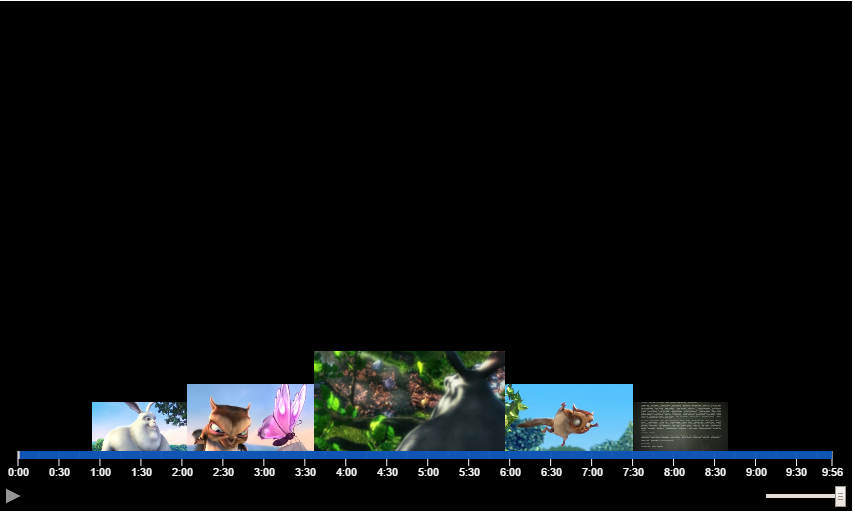
\includegraphics[width=0.7\textwidth]{videoBrowserBeginning.png}
	\caption{Die 5 Keyframes des Toplevels}
	\label{beginning}
\end{figure}

Man kann nun bei dem Keyframe, über das man den Mauszeiger gerade hat, eine Ebene tiefer gehen, indem man mit der Maus reinzoomt (scrollt). Zoomt man wieder heraus, gelangt man wieder zur vorherigen Ebene (siehe Abb. \ref{zoomedIn}). 

\begin{figure}[ht!]
	\centering
  	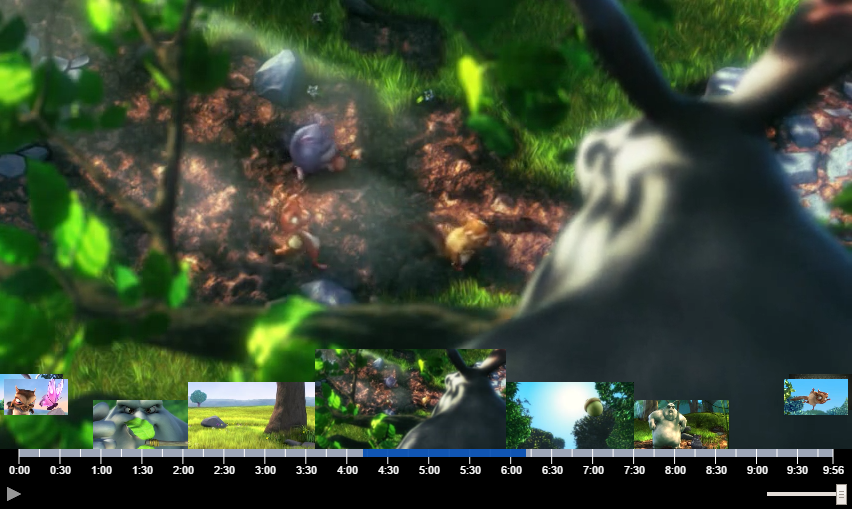
\includegraphics[width=0.7\textwidth]{videoBrowserZoomIn.png}
	\caption{Die 5 Keyframes und die Stapel der Nachbarclusters des zweiten Levels}
	\label{zoomedIn}
\end{figure}

Auf der Timeline am unteren Rand des Videos wird der Bereich im Video blau angezeigt, zu denen die Keyframes gehören. Insgesamt können 3 verschiedene Level angezeigt werden. Durch klicken auf die Stapel links und rechts neben den 5 Keyframes werden die Nachbarcluster von dem aktuellen Level angezeigt. 

Durch Klicken auf einen Keyframe wird das Video an der entsprechenden Position abgespielt. Mittels der Play/Pause Controls kann das Video abgespielt und gestoppt werden. Rechts unterhalb des Videos gibt es zudem noch einen Lautstärkeregler.


\end{document}
